% Chapter 2
\setlength\topmargin{8mm}
\onehalfspacing
\chapter{Funcionament} % Main chapter title

\label{Chapter2} % For referencing the chapter elsewhere, use \ref{Chapter1} 

\rhead[\emph{Disseny, programació i implementació d'un robot de dibuix amb Arduino}]{\thepage}
\lhead[\thepage]{\emph{Disseny, programació i implementació d'un robot de dibuix amb Arduino}}

%----------------------------------------------------------------------------------------



%----------------------------------------------------------------------------------------
\section{Motor pas a pas}
\subsection{Per què un motor pas a pas?}

Els motors pas a pas o “steppers”, són els motors ideals per controlar el moviment de les rodes del robot. En primer lloc ofereixen la possibilitat de rotar en les dues direccions, fet imprescindible per poder realitzar qualsevol trajectòria. La seva precisió angular és molt elevada, fet que permet coneixer en tot moment i amb exactitud quants graus ha girat el motor i per tant el moviment que han realitzat les rodes i, en definitiva, el robot. És un motor fàcil de controlar, amb el qual es pot minimitzar l'error comés gràcies a la seva excel·lent precisió, és pot controlar la seva velocitat i, per acabar, un altre avantatge que presenta és que quan el motor està parat, si rep corrent, ofereix una parell de resitència contra la rotació de l'eix, fet que evita que giri quan no ho ha de fer. 


\subsection{Funcionament}
El funcionament del motor pas a pas es bassa en la transformació d'impulsos elèctrics en “steps” o passos del motor, que són rotacions angulars exactes de l'eix. Típicament poden presentar 12, 24, 72, 144, 180 o 200 passos per volta i això significa que per cada impuls elèctric la seva rotació és de 30, 15, 5, 2.5, 2 o 1.8 graus respectivament. 


Presenta dues parts principals, l'estator, que esta format per bobines amb les quals s'indueix un camp magnètic al fer-hi passar corrent elèctric, i el rotor, que consisteix essencialment en un imant permanent rotatori, atret pel camp magnètic creat per l'estator. 


Al fer passar corrent per una de les bobines de l'estator es crea una polaritat i per tant s'orienta el rotor en funció d'aquesta polaritat, ja que sempre buscarà l'estabilitat magnètica entre els seus pols. Quan canvia l'excitació de l'estator, canvien els pols magnètics i per tant el rotor es reorienta. D'aquesta manera, al anar variant el pas del corrent per les bobines, es provoca un moviment circular del rotor molt precís, del qual es pot controlar la velocitat i el sentit de gir. 


\subsection{Tipus de motors pas a pas}
En funció de la connexió i la forma d'excitació de les  bobines, es pot diferencia entre dos tipus de motors pas a pas diferents, els unipolars i els bipolars.


\subsubsection{Unipolars}
El corrent que passa per les bobines de l'estator d'un motor pas a pas unipolar sempre va en el mateix sentit. Normalment tenen 5 o 6 cables de sortida, 6 si el cable d'alimentació comú de cada par de bobines va per separat i 5 si va junt. És més senzill de controlar ja que sempre es té el cable d'alimentació i cada pas es realitza al connectar a terra els altres cables amb un ordre determinat.

\subsubsection{Bipolars}
A diferencia dels unipolars aquests motors només presenten 4 cables de sortida, no tenen un comú d'alimentació. El seu funcionament es bassa en el canvi del sentit de circulació del corrent per les bobines en funció de la tensió, fet que provoca una diferència de polaritat que fa girar el rotor. Per tal de controlar-lo, és necessari utilitzar dos ponts H per poder invertir el sentit del corrent que passa per les dues bobines. 


\subsection{Modes de funcionamet}
Existeixen diferents seqüencies per aconseguir el moviment del motor, que dependrà de quines bobines estan excitades, en el cas dels motors unipolars, i en la direcció del corrent en els bipolars. 


\subsubsection{Seqüencia d'una fase}
Aquesta seqüencia consta de l'excitació d'una sola bobina fet que provoca un pas sencer del motor com es mostra a la imatge.  
\begin{figure}[H]
	\centering
	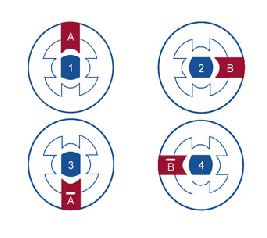
\includegraphics[scale=1.2]{Sequencia_1_fase.eps}
	\caption{Sequencia d'una fase.}
	\label{fig:1fase}
\end{figure}
La seva expressió en forma de taula és la següent:
\begin{table}[H]
	\begin{center}
		\begin{tabular}{|c||c|c|c|c|}
			\hline
			Pas & A & B & -A & -B \\
			\hline \hline
			1 & 1 & 0 & 0 & 0 \\ \hline
			2 & 0 & 1 & 0 & 0 \\ \hline
			3 & 0 & 0 & 1 & 0 \\ \hline
			4 & 0 & 0 & 0 & 1 \\ \hline
		\end{tabular}
		\caption{Seqüencia d' fase.}
		\label{tabla:1fase}
	\end{center}
\end{table}

\subsubsection{Seqüencia de dos fases}
Igual que a la seqüencia anterior, s'aconsegueix un pas per cada un dels estats de la sèrie, però la gran diferència és que per aconseguir-ho s'exciten dues bobines alhora, fet que provoca que la força d'atracció augmenti i aconsegueixi un millor parell de resistència. 
\begin{figure}[H]
	\centering
	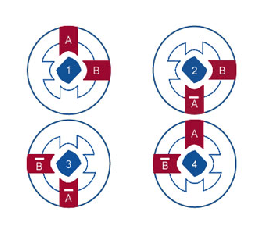
\includegraphics[scale=1.2]{Sequencia_2_fases.eps}
	\caption{Sequencia de dos fases.}
	\label{fig:Sequencia de dos fase}
\end{figure}
La seva expressió en forma de taula és la següent:
\begin{table}[H]
	\begin{center}
		\begin{tabular}{|c||c|c|c|c|}
			\hline
			Pas & A & B & -A & -B \\
			\hline \hline
			1 & 1 & 1 & 0 & 0 \\ \hline
			2 & 0 & 1 & 1 & 0 \\ \hline
			3 & 0 & 0 & 1 & 1 \\ \hline
			4 & 1 & 0 & 0 & 1 \\ \hline
		\end{tabular}
		\caption{Seqüencia de dos fases.}
		\label{tabla:2fase}
	\end{center}
\end{table}


\subsubsection{Seqüencia half step }
Amb una combinació de les dues anteriors, aconseguim que per cada estat de la sèrie el motor realitzi un gir de mig pas, i per tant aconsegueixi un moviment més petit. El seu funcionament es basa en l'excitació d'una sola bobina i de dues alhora de forma seqüencial com es mostra  a la figura.

\begin{figure}[H]
	\centering
	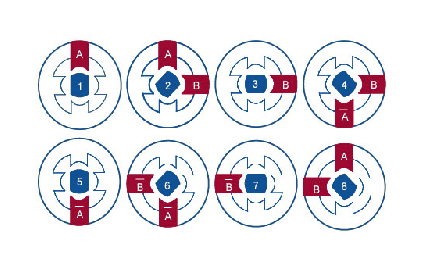
\includegraphics[scale=1.2]{Sequencia_halfstep.eps}
	\caption{Sequencia half step.}
	\label{fig:Sequencia half step}
\end{figure}
La seva taula de funcionament és la següent: 
\begin{table}[htbp]
	\begin{center}
		\begin{tabular}{|c||c|c|c|c|}
			\hline
			Pas & A & B & -A & -B \\
			\hline \hline
			1 & 1 & 0 & 0 & 0 \\ \hline
			2 & 1 & 1 & 0 & 0 \\ \hline
			3 & 0 & 1 & 0 & 0 \\ \hline
			4 & 0 & 1 & 1 & 0 \\ \hline
			5 & 0 & 0 & 1 & 0 \\ \hline
			6 & 0 & 0 & 1 & 1 \\ \hline
			7 & 0 & 0 & 0 & 1 \\ \hline
			8 & 1 & 0 & 0 & 1 \\ \hline	
		\end{tabular}
		\caption{Seqüencia mig pas (half step).}
		\label{tabla:hal step}
	\end{center}
\end{table}

\subsubsection{Microstepping}

L'objectiu del microstepping és aconseguir un moviment de rotació més suau, reduint els moviments bruscos entre passos del motor, augmentant el nombre de passos. Per aconseguir-ho s'utilitza un controlador, en aquest cas el driver explicat a l'apartat (\ref{sec:driver}), que idealment envia corrent en ones sinusoïdals enlloc d'impulsos. Es creen dos ones sinusoïdals desfasades 90º entre elles, una per cada bobina del motor, aconseguit així que quan a una bobina el corrent augmenta a l’altre decreix de la mateixa manera, creant un moviment perfecte del motor. 

A la realitat aquestes ones no són sinusoïdals perfectes, sinó que són ones esglaonades. Això provoca un augment de passos per volta del motor, en aquest cas es pot aconseguir multiplicar els passos per 2, 4 o 8 assolint un màxim de 1600 passos per volta. A la figura (\ref{fig:Microstepping}) es pot observar un exemple d’ona encarregada del microstepping. 

\begin{figure}[H]
	\centering
	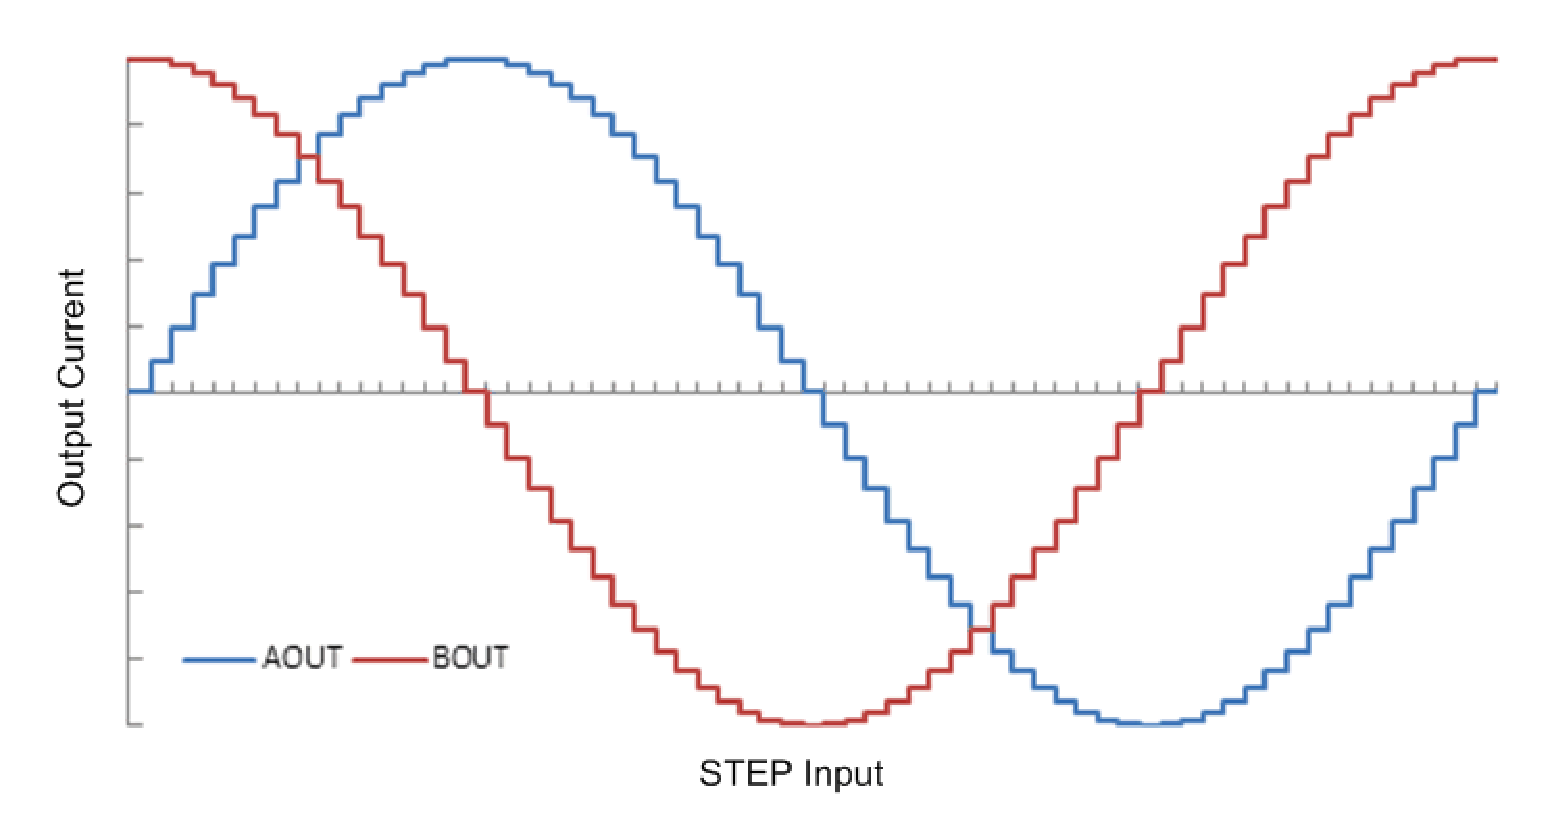
\includegraphics[scale=0.5]{OnaMicrostepping.eps}
	\caption{Ona sinusoïdal del microstepping.}
	\label{fig:Microstepping}
\end{figure}

\subsection{Alternatives}
Alhora de triar quins serien els motors adequats pel moviment del robot s'ha estudiat 3 opcions valides per fer-ho, el motor pas a pas, el motor de corrent continu i el servo-motor de rotació continua. S'ha escollit el motor pas a pas ja que el control de posició és bàsic pel funcionament del robot, i és l'únic que el pot assegurar sense la utilització d'un encoder i és el més fàcil de controlar. En els casos del motor de corrent continu i el servomotor de rotació continua, el seu funcionament es bassa en el control de la velocitat de rotació de l'eix segons la tensió o els impulsos del senyal de control respectivament, i per tant controlar la posició és molt més complicat. 


\subsection{Motor escollit: Nema 14}
Per escollir un motor pas a pas s'han estudiat els diferents models de la família NEMA i s'ha escollit entre el NEMA14 i el NEMA17 ja que són els que presenten les prestacions idònies pel moviment que es vol realitzar. Finalment la decisió s'ha decantat cap al NEMA14 ja que és més petit i té menys pes, la qual cosa permet adaptar-lo millor al prototip i realitzar un model amb unes dimensions més petites i òptimes. 

\begin{figure}[H]
	\centering
	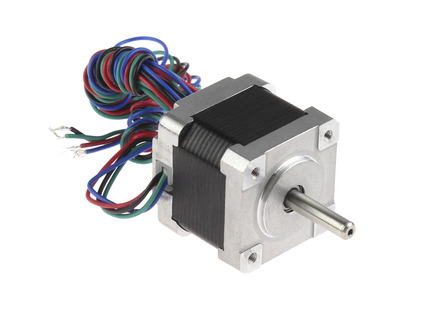
\includegraphics[scale=2]{NEMA14}
	\caption{Motor NEMA14.}
	\label{fig:NEMA14}
\end{figure}

El NEMA14 és un motor pas a pas bipolar amb les següents característiques: 

\begin{table}[htbp]
	\begin{center}
		\begin{tabular}{|c|c|}
			\hline
			
			Tensió nominal/fase & 2,7 V  \\ \hline
			Corrent nominal/fase & 1.0 A  \\ \hline
			Resistència/fase & 2,7 $\Omega$  \\ \hline
			Par de retenció & 1,4 Kg·cm  \\ \hline
			Número de cables & 4  \\ \hline
			Pes & 0,18 Kg  \\ \hline
			Àngle de pas & 1,8º  \\ \hline
			Passos per volta & 200  \\ \hline
		\end{tabular}
		\caption{Característiques del motor NEMA14.}
		\label{tabla:NEMA14}
	\end{center}
\end{table}



\section {Driver controlador del motor}\label{sec:driver}

\subsection{Controlador: Easy Driver A3967}

Els motors pas a pas bipolars necessiten un canvi de sentit en el flux de corrent  de les bobines per aconseguir així la seqüencia de fases desitjada per realitzar el moviment. A part d'això, com que els motors estan controlats per un microcontrolador Arduino UNO, s'ha de controlar la intensitat del corrent ja que podria fer malbé la placa. És per aquesta raó que s'ha decidit utilitzar un controlador que es basa en dos ponts H, un per cada bobina del motor, un dispositiu que suporta el flux bidireccional de corrent inversa i permet  canviar-lo de sentit.


Un pont H està format per 4 interruptors connectats com a la figura (\ref{fig:ponth})que permet fer passar el corrent per la bobina en un sentit o en un altre en funció de quina combinació d'interruptors s'utilitza, evitant així treballar amb voltatges negatius.

\begin{figure}[H]
	\centering
	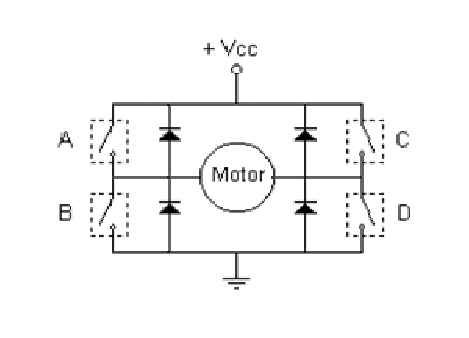
\includegraphics[width=0.40\linewidth]{PontH.eps}
	\caption{Connexió en pont H.}
	\label{fig:ponth}
\end{figure}

El seu funcionament és simple, i funciona per parelles d'interruptors que poden ser transistors bipolars, jfets, mosftes o alguna combinació entre ells. Si es tanquen els interruptors A i D el corrent circula en un sentit de la bobina i si al contrari els que es tanquen són B i C el corrent circula en l'altre sentit. Les combinacions A i B o C i D són perilloses pel circuit ja que crearien un curtcircuit. Els díodes són de protecció, ja que l'efecte inductiu de les bobines podria cremar el circuit un cop desconnectat.


\subsubsection{Easy Driver A3967}
Per facilitar el control dels motors pas a pas utilitzats, s'ha decidit utilitzar dos controladors Easy Driver A3967 que facilitarà el control i la programació dels motors i actuara com etapa de potència per no sobrecarregar l'Arduino amb la potencia requerida pel motor.


Com ja s'ha explicat, els motors pas a pas funcionen amb el canvi d'excitació de les bobines que el conformen, i cada parell de bobines te el seu parell de cables per fer-ho. La idea principal d'aquest driver o controlador és facilitar la feina i encarregar-se de l'alimentació dels motors, permetent així a l'usuari controlar el motor a través de només dos pins digitals de l'Arduino, l'STEP, que defineix un pas per cada pujada del pin i el DIR, que defineix el sentit de rotació del motor. 


A la següent imatge es mostra la distribució de les diferents entrades amb les que compta el controlador:

\begin{figure}[H]
	\centering
	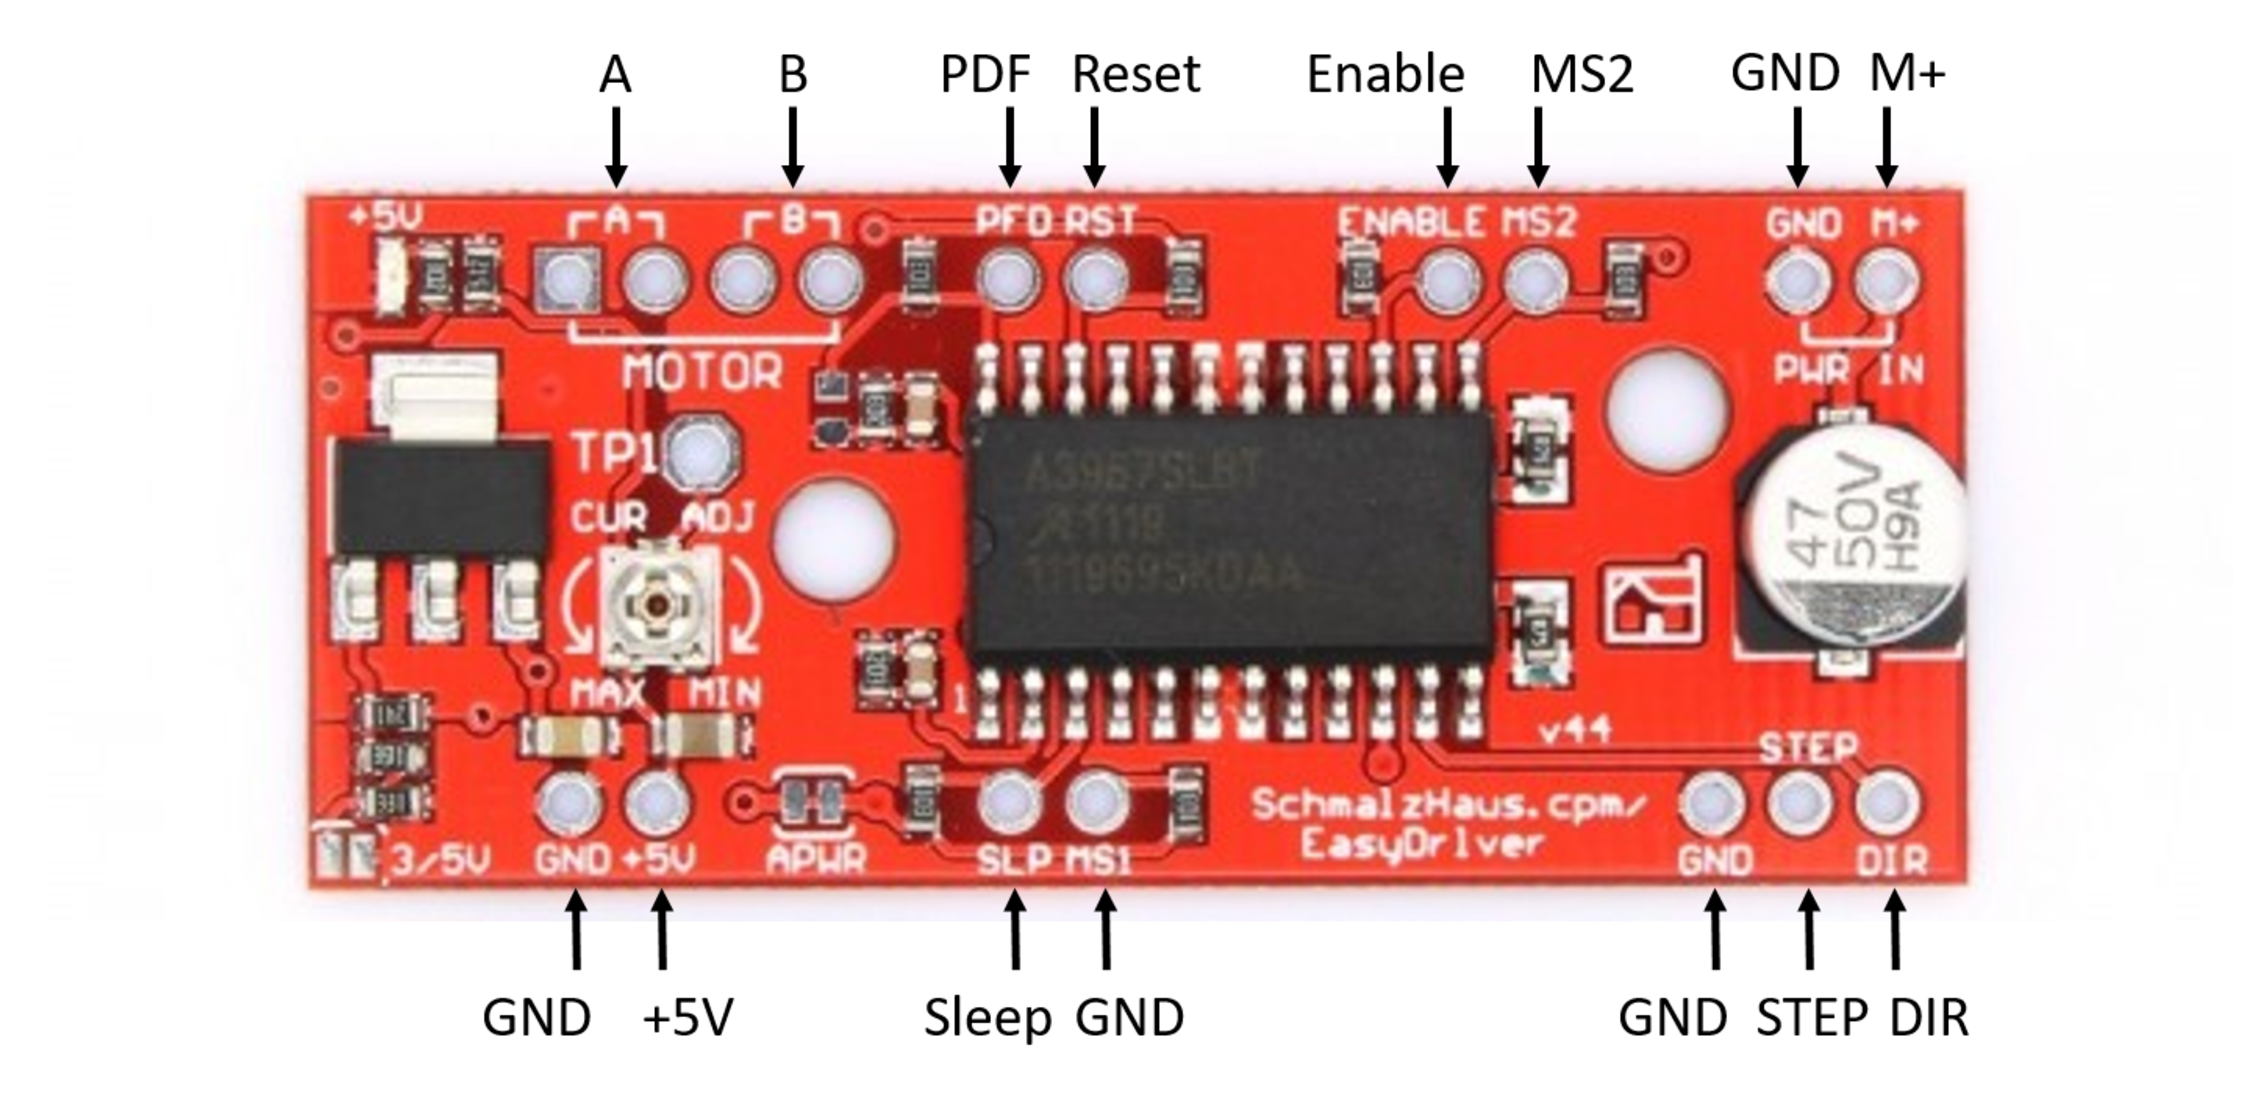
\includegraphics[width=1.00\textwidth]{PinsA3967.eps}
	\caption{Pins del driver A3967.}
	\label{fig:PinsA3967}
\end{figure}


Els pins principals i imprescindibles són els següents:


\begin{itemize}
	
	\item	A i B: Aquestes son les entrades dels 4 cables del motor, s'ha de connectar tenint en compte els dos parells de bobines diferents, una al als pins A i l'altre als pins B. 
	
	\item GND: Hi ha tres pins amb aquest nom i són la connexió a terra necessària a qualsevol circuit electrònic.
	
	\item STEP: Connectat a un pin digital d'Arduino, es l'encarregat de realitzar els passos del motor. A cada pujada de 0 a 5V, ordena al motor realitzar un pas. 
	
	\item DIR: Igual que l'STEP, va connectat a un pin digital d'Arduino (0-5V) i defineix segon el seu estat (high/low) la direcció del motor.
	
	\item M+: És l'entrada positiva de la font d'alimentació del motor i es recomana alimentar-la a un màxim de 12V. L'entrada negativa de la font es connecta al pin GND del costat.
	
\end{itemize}

La resta de pins permeten modificar el comportament del motor, però són opcionals:

\begin{itemize}
	
	\item MS1 i MS2: Aquests pins són els encarregats del microstepping. Poden reduir l'angle del pas i per tant augmentar la precisió de moviment del robot ja que redueixen moviment per pas. Hi ha 4 opcions de funcionament en funció de la connexió d'aquests dos pins que poden ser 0V (low) o 5V (high). El pas normal o full-step s'aconsegueix amb la combinació low/low, el mig pas o half-step amb high/low, un quart de pas o quarter-step amb low/high i un vuitè de pas o eight-step amb high/high. Per defecte la connexió és high/high, i per tant divideix el pas per 8. 
	
	\item Enable: És un input connectat com a low que elimina les sortides si es canvia a high.
	
	\item Reset: És un input connectat com a high que quan es canvia a low torna el controlador a la configuració inicial. 
	
	\item Sleep: És un input connectat com a high que minimitza el consum dels motors quan aquests no s'utilitzen si es canvia a low.
	
	\item +5V: Output de 5V que es pot utilitzar per alimentar components que funcionin a baixa corrent. 
	
	\item PDF: Aquest pin no s'utilitza, controla el mode de decadència del corrent de sortida.
	
\end{itemize}


\section {Servomotor}

\subsection{Quina és la seva funció?}

El servomotor és l’encarregat d’accionar el mecanisme per aixecar i baixar l’element de dibuix, en aquest cas el retolador, i, que per tant, permetrà a l’usuari decidir quins trams de la trajectòria formen part del dibuix i quins són moviments d’orientació i posicionament, els quals, gracies a aquest, no quedaran representats ja que no formen part del disseny. El funcionament del mecanisme d’elevació esta format pel servomotor que al rotar acciona una palanca unida al eix com a element terminal que, alhora, provoca un moviment vertical d’una placa plana unida al bolígraf que es desplaça per una guia.  

\subsection{Funcionament}

Els servos són un tipus de motors molt utilitzats en la robòtica gràcies a la seva gran precisió  angular en el posicionament, ja que permeten controlar la posició de l’eix en tot moment. Està dissenyat per posicionar-se en un rang determinat de posicions angulars (normalment de 0º a 180º), amb el qual es pot controlar el gir i la velocitat de rotació. Un cop realitzada la rotació de l’eix, el propi servo produeix un parell de resistència contra la rotació per mantenir estable la posició. També existeixen servos de rotació continua, però aquests no tenen control sobre la posició del mateix ja que, per tal de permetre la rotació continua s'elimina el potenciòmetre encarregat de tancar el llaç de control de la posició.

La composició d’un servomotor es bassa, normalment, en 4 elements fonamentals: 
\begin{itemize}

	\item	Motor de corrent continua: És l’encarregat de moure el motor, produeix una rotació de l’eix al aplicar-hi un corrent i es pot canviar el sentit de rotació aplicant el corrent invers.
	
	\item	Tren d’engranatges: Són un conjunt d’engranatges reductors que actuen per reduir la velocitat de sortida de l’eix del motor de corrent continua i brindar un parell més elevat per mantenir estable la posició.
	
	\item	Potenciòmetre: Es col·loca a la sortida de l’eix del motor de corrent continua per controlar la posició angular i així tancar el llaç de control. És pot eliminar i convertir el servo en un servo de rotació continua, però llavors es perd el control de la posició ja que el llaç de control quedaria obert.
	
	\item	Circuit de control:  Circuit electrònic encarregat de tancar el llaç de control comparant la senyal d’entrada amb la senyal de sortida mesurat pel potenciòmetre. Compara aquestes dues senyals per calcular l’error i corregir-lo, per tant un servo motor és un sistema de llaç tancat com el que es mostra a la figura. 
	
\end{itemize}

La connexió del servo és realitza a partir dels 3 cables que presenta, dos cables d'alimentació (positiu i negatiu) connectats a la font d’alimentació entre 4,8 i 6 V i un senyal de control per definir la posició mitjançant un senyal modulat per amplada de pols (PWM).

Mitjançant un microcontrolador, en el aquest cas un Arduino UNO, s’envia un senyal de polsos quadrats (PWM) al motor i, depenent de l’amplada del propi pols, el circuit de control posiciona l’eix a l’angle desitjat. Per la majoria de servos el senyal de control és el mateix, amb polsos quadrats d’entre 15 i 25 mil·lisegons de cicle de treball i l’angle depèn de l’amplitud del pols seguint l’exemple de la imatge. 
\begin{figure}[H]
	\centering
	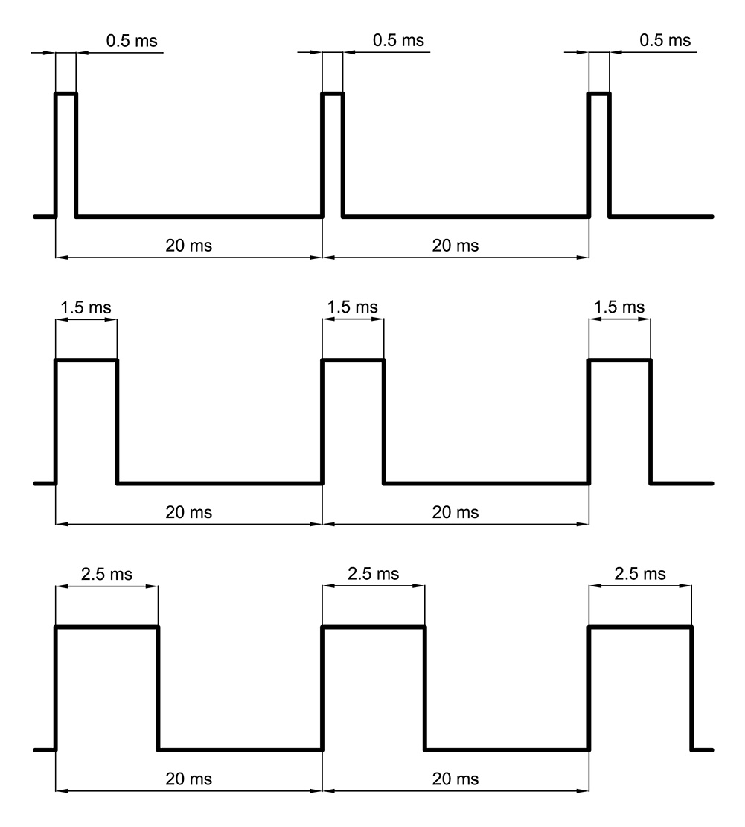
\includegraphics[scale=0.5]{entrada-servo.png}
	\caption{Exemples de senyal d'entrada del servomotor.}
	\label{fig:entradaservo}
\end{figure}

Amb la rotació del propi motor es posiciona el potenciòmetre permeten d’aquesta manera controlar i corregir l’error, per tant tancar el llaç de control entre el senyal d’entrada i el senyal de sortida llegit com la posició del potenciòmetre. 

\begin{figure}[H]
	\centering
	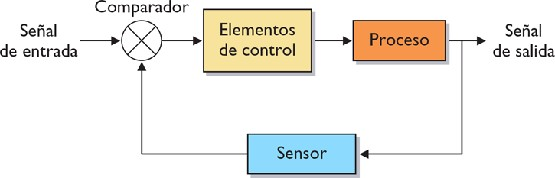
\includegraphics[scale=0.6]{llac-servo}
	\caption{Llaç de control del servomotor. (provisional)}
	\label{fig:llacservo}
\end{figure}

Existeixen 2 tipus diferents de servomotors, els analògics i els digitals. Els digitals tenen millors característiques, millor resolució, resposta més ràpida, una acceleració més suau durant el moviment i un parell més elevat en estat estacionari. Però, per altra banda, tenen un consum més elevat ja que treballen a una freqüència deu vegades majors a la dels analògics i el seu preu és molt més elevat. 

\section{Bateria}

L’objectiu del projecte era dissenyar un robot autònom, i per aquesta raó s’ha decidit incorporar una bateria que subministra l’energia necessària als dos motors així com al microcontrolador Arduino Uno. Després de les proves inicials es va decidir separar les fonts dels dos motors per evitar d’aquesta manera un mal repartiment de la potencia i complir en tot moment amb les exigències energètiques d’ambdós motors. 

S’ha optat per escollir una bateria externa recarregable de la marca Proda de 10000 mAh per dos motius, en primer lloc perquè ofereix dues sortides de corrent de 5V a 1 i 2A respectivament i pot per tant alimentar els dos motors per separat, i perquè s’havia comprat abans de començar el projecte i no calia adquirir-ne una altra. 

És una bateria de polímer d’ions de liti (LiPo) que permet emmagatzemar una gran càrrega d’energia i per tant permetrà operacions de llarga durada del prototip. L’avantatge que presenta és, com ja s’ha explicat, que té dos canals amb els quals és possible alimentar tots els components del robot des d'una mateixa font d'alimentació. Així doncs, el canal de sortida de 5V i 2A s’encarrega d’alimentar el motor dret del robot i el microcontrolador Arduino UNO (que tanmateix el propi Arduino subministra el corrent necessari pel funcionament del mòdul Bluetooth), mentre que el de 5V i 1A alimenta el motor esquerra i el servo. També conté una petita pantalla per mostrar la càrrega actual de la bateria i que així l’usuari sàpiga en tot moment si cal recarregar-la. Per altre banda, el desavantatge que presenta és el seu elevat pes (170 grams), tot i que després de les proves inicial es va comprovar que els motors eren capaços de moure aquesta càrrega sense problemes. 

\begin{figure}[H]
	\centering
	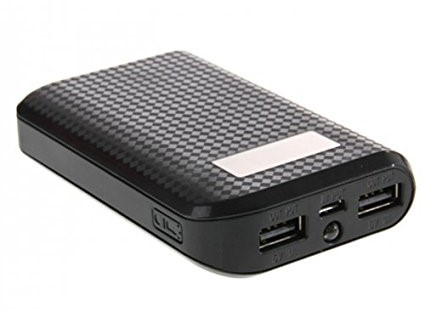
\includegraphics[scale=0.4]{bateria.png}
	\caption{Imatge de la bateria utilitzada.}
	\label{fig:bateria}
\end{figure}

\section{Retolador} \label{sec:retolador}

Com a element de dibuix s’ha escollit un retolador Edding 1200. És un retolador que es pot compra a qualsevol papereria, amb una amplia gamma de colors i un funcionament excel·lent. Les principals característiques que el fan perfecte per aquesta funció són el seu perfil circular de diàmetre constant que permet el lliscament dins de la guia de plàstic fixe al xassís del robot i que la seva tinta s’asseca de forma immediata després de pintar el paper, evitant així que les rodes puguin fer malbé el dibuix si passen per sobre el traçat i arroseguen la tinta si encara no s'ha assecat. Amb el seu propi pes més el del suport que l'aguanta és suficient per dibuixar la línia sobre el paper i no ofereix resistència per fricció, i per tant no afecta negativament a la trajectòria del robot. 

Com s’explicarà més endavant a l'apartat (\ref{sec:suportmobil}), s’ha creat un suport per tal d’aixecar-lo quan la trajectòria del robot sigui de posicionament i la seva posició és al centre de l’eix coaxial als eixos dels dos motors, facilitant d’aquesta manera el control de la seva trajectòria. 

\begin{figure}[H]
	\centering
	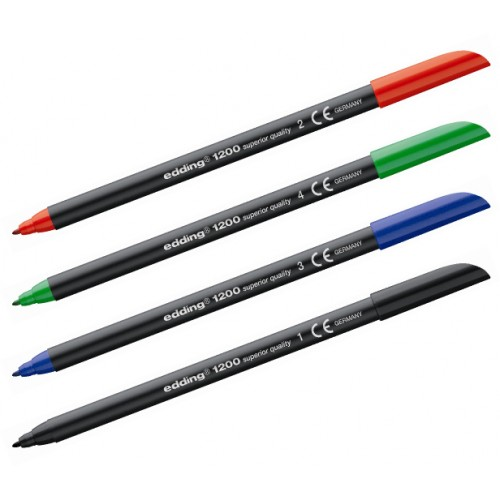
\includegraphics[scale=0.3]{retolador.png}
	\caption{Imatge de la bateria utilitzada.}
	\label{fig:retolador}
\end{figure}